\documentclass[letterpaper,12pt]{article}
%\usepackage{harvard}
%\usepackage{subfigure}
%\usepackage[active]{srcltx}
\usepackage{graphicx}
\usepackage{pdflscape}
\usepackage{amsmath}
\usepackage{amsthm}
\usepackage{lscape}
\usepackage{enumerate}
\usepackage{float}
\usepackage{grffile}
\usepackage{relsize}
\usepackage{tablefootnote}
\usepackage{footnote}
\usepackage{sectsty}
\usepackage{xcolor}
\usepackage{caption}
\usepackage{color}
\usepackage{natbib}
\usepackage{multirow}
\usepackage{bbm}
\usepackage[T1]{fontenc}
\usepackage[multiple]{footmisc}
\usepackage{appendix}
\usepackage{times}
\usepackage{relsize}
\usepackage{caption}
\usepackage{newtxtext,newtxmath}
\usepackage{enumitem}


%%%%%%%%%%%%%%%%%%%%%%%%%%%%%%%%%%%%%%%%%%%%%%%%%%%%%%%%%%%%
%%%   Title Page Information
%%%%%%%%%%%%%%%%%%%%%%%%%%%%%%%%%%%%%%%%%%%%%%%%%%%%%%%%%%%%
\title{\vspace{-1in}ECON311: Midterm}
\author{Leandro Freylejer}
\date{}

%%%%%%%%%%%%%%%%%%%%%%%%%%%%%%%%%%%%%%%%%%%%%%%%%%%%%%%%%%%%
%%%   Double and Single Space Commands
%%%%%%%%%%%%%%%%%%%%%%%%%%%%%%%%%%%%%%%%%%%%%%%%%%%%%%%%%%%%
\newlength{\defbaselineskip}
\setlength{\defbaselineskip}{\baselineskip}
\newcommand{\setlinespacing}[1]{\setlength{\baselineskip}{#1 \defbaselineskip}}
\newcommand{\doublespacing}{\setlength{\baselineskip}{1.3 \defbaselineskip}}
\newcommand{\singlespacing}{\setlength{\baselineskip}{1\defbaselineskip}}
\renewcommand{\thesubsection}{\arabic{subsection}}
\newtheoremstyle{dotlessS}{}{}{\itshape}{}{\color{dg}\bfseries}{}{ }{}
\theoremstyle{dotlessS}
\newtheorem{theorem}{Theorem}
\newtheorem{lemma}{Lemma}
\newtheorem{proposition}{Proposition}
\newtheorem{assumption}[theorem]{Assumption}
\newtheorem{corollary}{Corollary}
\newtheorem{definition}{Definition}
\newenvironment{example}[1][Example]{\begin{trivlist}
\item[\hskip \labelsep {\bfseries #1}]}{\end{trivlist}}
\newenvironment{remark}[1][Remark]{\begin{trivlist}
\item[\hskip \labelsep {\bfseries #1}]}{\end{trivlist}}

\newcommand\Pitem{%
  \addtocounter{enumi}{-1}%
  \renewcommand\theenumi{\arabic{\enumi}'}%
  \item%
  \renewcommand\theenumi{\arabic{enumi}}%
}

%%%%%%%%%%%%%%%%%%%%%%%%%%%%%%%%%%%%%%%%%%%%%%%%%%%%%%%%%%%%
%%%   Set Margins Here
%%%%%%%%%%%%%%%%%%%%%%%%%%%%%%%%%%%%%%%%%%%%%%%%%%%%%%%%%
\textwidth=6.5in
\textheight=9in
\oddsidemargin=0.10in
\evensidemargin=0.10in
\topmargin=-0.5in
%\parskip=3pt

%%%%%%%%%%%%%%%%%%%%%%%%%%%%%%%%%%%%%%%%%%%%%%%%%%%%%%%%%%%%%
%%%   Actual Document Begins Here
%%%%%%%%%%%%%%%%%%%%%%%%%%%%%%%%%%%%%%%%%%%%%%%%%%%%%%%%%%%%%
\begin{document}


\pagenumbering{arabic}
\maketitle
\noindent There are six questions in this exam for a total of 60 points. You must show all your work to get full marks. You are allowed a calculator. Good Luck!!!
\section{Part I: Short-Answer Questions}

\subsection*{Question I: Solow Model (6 points)}
Refer to Figure 1, where c refers to consumption per worker and y to output per worker, when answering the following question.
\begin{figure}[H]
\centering
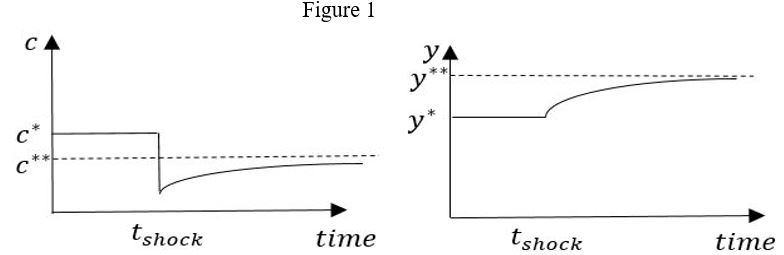
\includegraphics[scale=.75]{Solow_model}
\end{figure}
Consider the Solow Model economy studied in class:
\begin{eqnarray*}
\begin{array}{ll}
\text{Production Function} &Y_t=\overline{A} \: \left(K_t\right)^{\frac{1}{3}} \: \left(\overline{L}\right)^{\frac{2}{3}}\\[1.4ex]
\text{Capital Accumulation} &K_{t+1}=I_t+(1-\overline{d}) \: K_t \\[1.4ex]
\text{Resource Constraint} &C_t+I_t=Y_t  \\[1.4ex]
\text{Allocation of Resources} &I_t=\overline{s} \: Y_t  \\[1.4ex]
\end{array}
\end{eqnarray*}
Use this model to show the shock at time $t_{shock}$ that best describes the transitional dynamics in Figure 1. To answer this question use the Solow diagram with total output.


\subsection*{Question II: Romer Model (8 points)}
Consider the following Romer economy: 
\begin{eqnarray*}
\begin{array}{ll}
\text{Production Function:} & Y_t=A_t  \: L_{Y_t} \\[1.4ex]
\text{Productivity:} & A_{t+1}=A_t+\overline{z} \: A_t \: L_{A_{t}}  \\[1.4ex]
\text{Allocation of labour:} & L_{A_{t}}=\overline{I} \: \overline{L}, \: \: \:  \: \: L_{Y_{t}}=(1-\overline{I}) \: \overline{L}  \\[1.4ex]
\end{array}
\end{eqnarray*}
Derive the rate of growth of output per person in the long-run equilibrium ($g_y$). Use the previous equation to explain the trade-off between long-run growth and the short-run level of consumption in this model. In your answer make sure to include a graph with output per person on the vertical axis (using a ratio scale) and time on the horizontal axis. Label your graph carefully.




\subsection*{Question III: Economic Growth}
Table I contains per capita real GDP for two countries: Argentina and Japan for the years 1950 and 2014.  
\begin{table}[H]
\begin{minipage}[h]{1\textwidth}
\centering
\caption*{Table I: Real GDP Per Capita in $\$$US}
\resizebox{6cm}{!}{%
\begin{tabular}{lll}
\hline
Country    & 1950    & 2014   \\
\hline
Argentina &2,890     &20,222  \\   
Japan       &2,616     &35,358  \\ 
\hline
\end{tabular}}
\end{minipage} 
\end{table}
\noindent Using the the three formulas for annual average growth rates: $y_{t+T}=y_t \: \: (1+\overline{g})^T$, $\overline{g}=\left(\frac{y_{t+T}}{y_t}\right)^{\frac{1}{T}}-1$ and $T=\frac{ln(y_{t+T}/y_t)}{\overline{g}}$, answer the following questions:
\begin{enumerate}[label=(\alph*)]
\item (3 points) Calculate the average annual growth rates for each country between 1950 and 2014. 
\item (3 points) Assume that the Argentine economy keeps growing at the same annual rate you found in part (a). How many more years from 2014 would it take for Argentina to reach the per capita real GDP levels of Japan in 2014? 
\item (4 points) Turkey had an average growth rate of $1.5\%$ over the same period. The Turkish and Argentine economies are expected to continue growing at the same average rates as in the 1950-2014 period respectively, and achieve the same level of per capita real GDP by 2024. Using this information, calculate the per capita real GDP of Turkey in 2014. 
\end{enumerate}     


\section{Part II: Long-Answer Questions}

\section*{Question I: Model of Production}
Suppose that total GDP in a country at a given year is given by the following production function:
\begin{eqnarray*}
Y_t=F(K_t, L_t, N_t)=\overline{A}(K_t)^{\frac{1}{4}}(L_t)^{\frac{1}{2}}(N_t)^{\frac{1}{4}} 
\end{eqnarray*}
where $N$ represents natural resources and all other variables are the same as in class. The introduction of $N$ expands the production model by allowing production to also depend on the natural resources available to produce in a country. 
\begin{enumerate}[label=(\alph*)]
\item (4 points) Does the previous production function exhibit constant, diminishing or increasing returns to scale? Explain.
\item (6 points) Suppose that labour and capital grow at the same constant rate, $g_K=g_L=g>0$, and that natural resources as well as productivity  are constant (i.e. $N_t=\overline{N}$, $A_t=\overline{A}$). Calculate the growth rates of GDP and GDP per capita as a function of $g$. Are these growth rates positive or negative? Carefully explain.
\item (6 points) Suppose now that labour, capital and TFP ($A$) grow at the same rate, , $g_K=g_L=g_A=g$, and that natural resources are constant (i.e. $N_t=\overline{N}$). Calculate the growth rates of GDP and GDP per capita. Are these growth rates positive or negative? Carefully explain. 
\end{enumerate}


\section*{Question II: Solow Growth Model (10 points)}

The economy of the country of Borduria is given by:
\begin{eqnarray*}
\begin{array}{ll}
\text{Production Function} & Y_t=\overline{A} \left(K_t\right)^{\frac{1}{3}} \left(\overline{L}\right)^{\frac{2}{3}}  \\[1.4ex]
\text{Capital Accumulation} & \Delta K_{t+1}=I_t-\overline{d}K_t  \\[1.4ex]
\text{Investment}            & I_t=\overline{s} Y_t    \\[1.4ex]
\text{Consumption}       & C_t=(1-\overline{s}) Y_t    \\[1.4ex]
\end{array}
\end{eqnarray*}
Suppose that there is a negative productivity shock in Borduria, in particular, $\overline{A}$ permanently decreases to $\overline{A}'$. Explain what happens to the economy over time (transition dynamics) and in the long run (steady state). In particular, discuss what happens to the levels of capital, GDP and consumption both at the new steady state as well as during transitions to the new steady state. To answer this question use both the Solow diagram with total output, and diagrams with time on the horizontal axis and each of these variables on the vertical axis.


\section*{Question III: Measuring the Macroeconomy (10 points)}
Refer to the Table II when answering the following question. In this economy, only two goods are produced: video games and pistachios.
\begin{figure}[H]
\centering
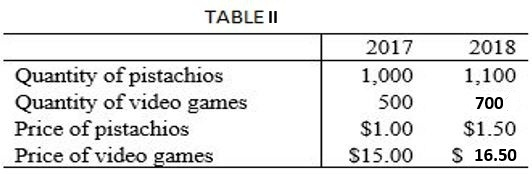
\includegraphics[scale=.7]{table_1}
\end{figure}
\noindent Using the GDP Deflator and the Laspeyres Quantity Index to calculate changes in Real GDP across time, calculate the inflation rate between 2017 and 2018. Does changing the benchmark year affect your result? Explain.   


\end{document}
